\section{Linear Regression for Multivariate Real World Data  $\And$ Bivariate Data}
The model implemented here makes use of a Gaussian Basis Function,
\begin{equation*}
    \mathbb{\phi}_j(\mathbf{x}) = \exp \left( {-\frac{(\mathbf{x} - \mu_j)^2}{\sigma^2}} \right)
\end{equation*}

\subsection{Experiments $\And$ Observations on Dataset 2:}

\subsubsection{RMS error comparison for varying dimensions and width of $\mathbb{\phi}(\mathbf{x})$:}

A total of 500 samples from the given bivariate dataset was chosen at random and divided in to training, validation and test data(70$\%$, 20$\%$ and 10$\%$). Using the training data thus generated an attempt is made to find the best model. At first the case without regularisation is considered. For each dimension of the gaussian basis function, different values of width has been experimented here. As can be concluded from the tables, a dimension of 75 and width of 10 seems to be optimal model for the regression task at hand. Also, one can observe over-fitting when the dimensions are increased to 340 and for width of 1. The value of training data, $E_{rms}$ is drastically lower than that of validation data.

{\rowcolors{3}{green!40!yellow!10}{green!0!yellow!30}
\begin{table}[hptb]
\begin{tabular}{ |p{1.5cm}|p{3cm}|p{3cm}| p{3cm}|  }
\hline
\multicolumn{4}{|c|}{$\mathbf{E}_{rms}$ values for dimension $25$ } \\
\hline
\rowcolor{lightgray} \textbf{Width} & $\mathbf{E}_{rms-train}$ & $\mathbf{E}_{rms-val}$ & $\mathbf{E}_{rms-test}$ \\
\hline
  1   &   $3.40 \times 10^4$   &  $6.42 \times 10^4 $        &     $4.16 \times 10^4 $   \\
 \hline
 10   &   $3.07 \times 10^3$  &  $4.12 \times 10^3 $          &     $3.17 \times 10^3 $   \\
 \hline
 50   &   $1.96 \times 10^5$  & $2.01 \times 10^5$          &         $2.08 \times 10^5$   \\
\hline
\end{tabular}
\label{table:8}
\end{table}
}
{\rowcolors{3}{green!40!yellow!10}{green!0!yellow!30}
\begin{table}[hptb]
\begin{tabular}{ |p{1.5cm}|p{3cm}|p{3cm}| p{3cm}|  }
\hline
\multicolumn{4}{|c|}{$\mathbf{E}_{rms}$ values for dimension $50$ } \\
\hline
\rowcolor{lightgray} \textbf{Width} & $\mathbf{E}_{rms-train}$ & $\mathbf{E}_{rms-val}$ & $\mathbf{E}_{rms-test}$ \\
\hline
  1   &   $2.70 \times 10^4$   &  $4.39 \times 10^4 $        &     $5.50 \times 10^4 $   \\
 \hline
 10   &   $3.33 \times 10^2$  &  $4.87 \times 10^2 $          &     $4.46 \times 10^2 $   \\
 \hline
 50   &   $7.01 \times 10^5$  & $6.86 \times 10^5$          &         $6.72 \times 10^5$   \\
\hline
\end{tabular}
\label{table:8}
\end{table}
}
{\rowcolors{3}{green!40!yellow!10}{green!0!yellow!30}
\begin{table}[hptb]
\begin{tabular}{ |p{1.5cm}|p{3cm}|p{3cm}| p{3cm}|  }
\hline
\multicolumn{4}{|c|}{$\mathbf{E}_{rms}$ values for dimension $75$ } \\
\hline
\rowcolor{lightgray} \textbf{Width} & $\mathbf{E}_{rms-train}$ & $\mathbf{E}_{rms-val}$ & $\mathbf{E}_{rms-test}$ \\
\hline
  1   &   $2.28 \times 10^4$   &  $3.56 \times 10^4 $        &     $4.79 \times 10^4 $   \\
 \hline
 10   &   $1.18 \times 10^2$  &  $1.47 \times 10^2 $          &     $1.34 \times 10^2 $   \\
 \hline
 50   &   $3.84 \times 10^5$  & $3.94 \times 10^5$          &         $4.05 \times 10^5$   \\
\hline
\end{tabular}
\label{table:8}
\end{table}
}
{\rowcolors{3}{green!40!yellow!10}{green!0!yellow!30}
\begin{table}[hptb]
\begin{tabular}{ |p{1.5cm}|p{3cm}|p{3cm}| p{3cm}|  }
\hline
\multicolumn{4}{|c|}{$\mathbf{E}_{rms}$ values for dimension $340$ } \\
\hline
\rowcolor{lightgray} \textbf{Width} & $\mathbf{E}_{rms-train}$ & $\mathbf{E}_{rms-val}$ & $\mathbf{E}_{rms-test}$ \\
\hline
  1   &   $1.01 \times 10^3$   &  $2.51 \times 10^4 $        &     $1.97 \times 10^4 $   \\
 \hline
 10   &   $2.74 \times 10^6$  &  $3.30 \times 10^6 $          &     $3.41 \times 10^6 $   \\
 \hline
 50   &   $5.22 \times 10^5$  & $5.29 \times 10^5$          &         $5.32 \times 10^5$   \\
\hline
\end{tabular}
\caption{Error comparisons for varying values of $\phi(\mathbf{x}) $  and width($\sigma$) for Dataset 2}
\label{table:8}
\end{table}
}

\newpage
\subsubsection{Effect of regularisation in case of over-fitting:}

As inferred from the previous section, the over-fit case of dimension 340 and width 1 is experimented for different values of $\lambda$, thus a regularisation term is added resulting in various models for fixed dimension and width. Both quadratic and tikhonov regulariser are experimented with here. This helps us to see the impact of regularisation in case of over-fitting. As can be seen from the error values, though adding a regulariser doesn't better fit the model but it helps in ruling out models which have essentially memorized the training data-set but perform poorily on test data set.

{\rowcolors{3}{green!40!yellow!10}{green!0!yellow!30}
\begin{table}[hptb]
\begin{tabular}{ |p{1.5cm}|p{3cm}|p{3cm}| p{3cm}|  }
\hline
\multicolumn{4}{|c|}{$\mathbf{E}_{rms}$ values for different data } \\
\hline
\rowcolor{lightgray} $\lambda$ & $\mathbf{E}_{rms-train}$ & $\mathbf{E}_{rms-val}$ & $\mathbf{E}_{rms-test}$ \\
\hline
  10e-5  &  $1.07 \times 10^3$       &       $2.517 \times 10^4$ & $1.979 \times 10^4$  \\
 \hline
  10e-3  &   $1.08 \times 10^3$       &       $2.520 \times 10^4$        &     $1.974 \times 10^4$     \\
 \hline
  10e-1  &   $1.17 \times 10^3$       &       $2.529 \times 10^4$       &     $1.983 \times 10^4$    \\
 \hline
  0  &    $1.01 \times 10^3$     &      $2.516 \times 10^4 $         &     $1.979 \times 10^4$      \\
  \hline
  10     &   $2.84 \times 10^4$   &        $3.852 \times 10^4$         &     $3.782 \times 10^4$      \\
  \hline
  10e+03   &   $5.11 \times 10^4$    &         $5.919 \times 10^4$      &      $6.081 \times 10^4$        \\
  \hline
  10e+05  &    $5.20 \times 10^4$  &         $6.001 \times 10^4$       &        $6.170 \times 10^4$      \\
\hline
\end{tabular}
\caption{Error comparisons for quadratic regularisation by varying $\lambda $  and fixed dimension =340 and width = 1 for Dataset 2}
\label{table:9}
\end{table}
}


{\rowcolors{3}{green!40!yellow!10}{green!0!yellow!30}
\begin{table}[hptb]
\begin{tabular}{ |p{1.5cm}|p{3cm}|p{3cm}| p{3cm}|  }
\hline
\multicolumn{4}{|c|}{$\mathbf{E}_{rms}$ values for different data } \\
\hline
\rowcolor{lightgray} $\lambda$ & $\mathbf{E}_{rms-train}$ & $\mathbf{E}_{rms-val}$ & $\mathbf{E}_{rms-test}$ \\
\hline
  10e-3  &   $1.007 \times 10^3$       &       $2.543 \times 10^4$        &     $1.970 \times 10^4$     \\
 \hline
  10e-1  &   $1.046 \times 10^3$       &       $3.088 \times 10^4$       &     $2.763 \times 10^4$    \\
 \hline
  0  &    $1.007 \times 10^3$     &      $2.516 \times 10^4 $         &     $1.979 \times 10^4$      \\
  \hline
  10     &   $3.161 \times 10^4$   &        $4.01 \times 10^4$         &     $3.930 \times 10^4$      \\
  \hline
  10e+03   &   $5.119 \times 10^4$    &         $5.920 \times 10^4$      &      $6.080 \times 10^4$        \\
  \hline
  10e+05  &    $5.204 \times 10^4$  &         $6.005 \times 10^4$       &        $6.170 \times 10^4$      \\
\hline
\end{tabular}
\caption{Error comparisons for tikhonov regularisation by varying $\lambda $  and fixed dimension =340 and width = 1 for Dataset 2}
\label{table:10}
\end{table}
}

\newpage
\subsubsection{Scatter Plots of Best Model}
Figure [\ref{fig:17}] shows the the scatter plot of predicted and actual target variable for the training and the test data.

\begin{figure}[h]
    \centering
    \begin{subfigure}[t]{0.50\textwidth}
        \centering
        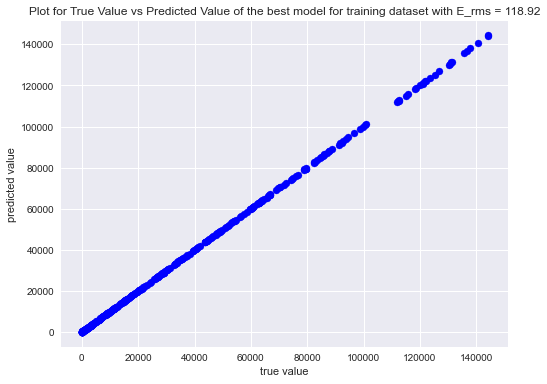
\includegraphics[height=1.6in]{Task3_new_images/batch500_tr.png}
        \caption{Training Data}
    \end{subfigure}%
    ~ 
    \begin{subfigure}[t]{0.50\textwidth}
        \centering
        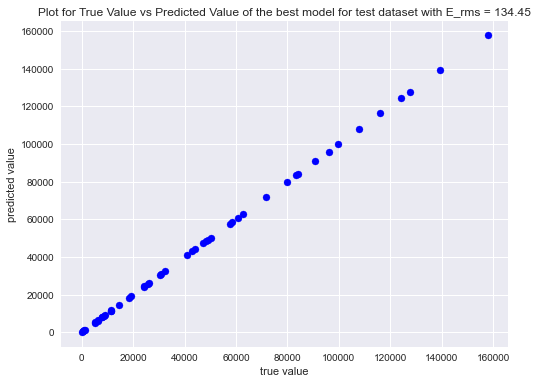
\includegraphics[height=1.6in]{Task3_new_images/batch500_test.png}
        \caption{Test Data }
    \end{subfigure}%
    \caption{Scatter Plot of the Gaussian Basis Function of the best performing model for Dataset 2}
    \label{fig:17}
\end{figure}

%%%%%%%%%%%%%%%%%%%%%%%%%%%%%%%%%%%%%%%%%%%%%%%%%%%%%%%%%%%%%%%%%%%%%%%%%%%%%%%%%%%%%%%%%%%%%%%%%%%%%%%%%%%%%%%%%%%%%%%%%%%%%%%%%%%%%%%%%%%%%%%%%%%%%%%%%%%%%%%%%%%%%%%%%%%%%%%%%%%%%%%%%%%%%%%%%%%%%%%%%%%%%%%%%%%%%%%%%%%%%%%%%%%%%%%%%%%%%%%%%%%%%%%%%%%%%%%%%%%%%%%%%%%%%%%%%%%%%%%%%%%%%%%%%%%%%


% \subsection{Experiments $\And$ Observations on Dataset 3:}

% \begin{figure}[!ht]
%     \centering
%         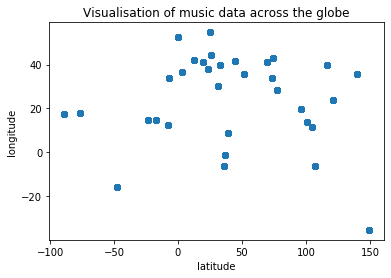
\includegraphics[height=3.2in]{Task 3 Images/Visualisation of music data across the globe.png}
%         \caption{Training Data}
% \end{figure}